\documentclass{article}

\usepackage[utf8]{inputenc}  % For encoding support
\usepackage{amsmath}         % For mathematical formatting
\usepackage{graphicx}        % For including images
\usepackage{xcolor}
\usepackage[a4paper, left=0.5in, right=0.5in, top=0.5in, bottom=0.5in]{geometry}  % Adjust margins here

\title{Compiler Design Notes}
\author{Ayush Raina}
\date{\today}

\begin{document}

\maketitle

\section*{Control Flow Analysis}
\subsection*{Why Control Flow Analysis?}
Helps to understand structure of Control Flow Graph (CFG), To detect loops in the CFG, Dominator Information,Dominator Frontier Information required for Single Static Assignment (SSA) form. Interval Information used in Data Flow Analysis, Control Dependence Information used in Parallelization.

\subsection*{Dominators}
\begin{enumerate}
    \item We write $(d \text{ dom } n)$ if every path from initial node $n_0$ to node $n$ passes through node $d$. A node dominates itself.
    \item Node $x$ strictly dominates node $y$ if $x$ dominates $y$ and $x \neq y$.
    \item $x$ is immediate dominator of $y$ if $x$ is closest strict dominator of $y$.
\end{enumerate}

\subsection*{Algorithm to find Dominators}
Let us denote the set of Dominators of node $n$ as $D(n) = OUT(n)$. These sets are very helpful to construct the dominator tree quickly. 
\begin{itemize}
    \item Start with $n_0$ such that $D(n_0) = \{n_0\}$.
    \item for each $n \in N - \{n_0\}$ do the following:
    \begin{itemize}
        \item First set $D(n) = N$.
        \item Take intersection of all the outsets of the predecessors of $n$ denoted by $IN(n) = \bigcap_{p \in pred(n)} OUT(p)$.
        \item $D(n) = IN(n) \cup \{n\}$.
    \end{itemize}

    \item Repeat until $D(n)$ stabilizes for all $n$.
\end{itemize}

\subsection*{Back Edges and Natural Loops}

\textbf{Back Edges: } Edges whose head dominates the tail are called back edges. To find the back edges, one easy way to look if opposing edges according to dominator tree is present in the graph. \\
\textbf{Natural Loops: } Given a back edge $(n,d)$, the natural loop of the edge is $d \cup $ all the nodes that reach $n$ without going through $d$. In this case $d$ is the header of the loop and dominates all the nodes in the loop.

\subsection*{Algorithm for finding the natural loop of a back edge} 
Let the back edge be $(n,d)$. Then initialize a empty stack. Push $n$ into the stack. Initialize a vector with $d$ in it. Then until the stack is empty, pop the top element and push its predecessors into the stack. If the predecessor is not in the vector, add it to the vector. Continue until the stack is empty. The vector now contains the natural loop.

\subsection*{Depth First Numbering of Nodes in a CFG}
We start a $DFS(n)$ from initial node $n_0$ where $n$ is total number of nodes. We mark a node to $n$ when it is last visit to that node. Last visit means that all the children of that node are visited and now this node will not be visited again. Then we decrement $n$ and continue the process. This way we can number the nodes in a CFG.

\begin{figure}[h]
    \centering
    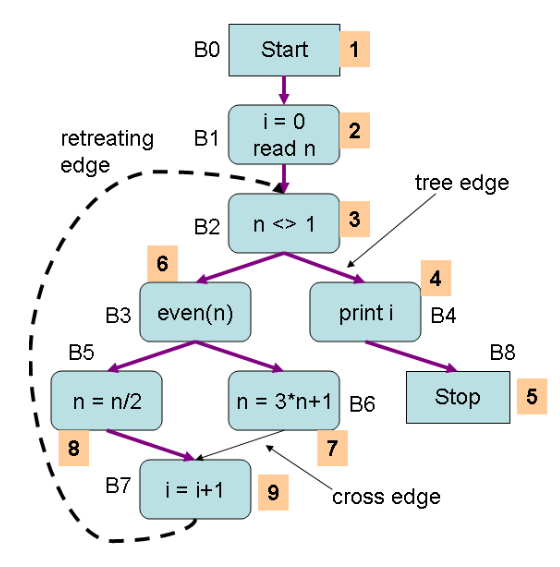
\includegraphics[width=0.5\textwidth]{Images/dfs1.png}
    \caption{DFS Numbering of Nodes}
    \label{fig:cfg}
\end{figure}

\newpage

\subsection*{Reducibility}
A flow graph $\mathcal{G}$ is reducible iff every back it can be partitioned into 2 disjoint sets of forward and back edges such that:

\begin{itemize}
    \item Forward edges form a DAG in which every node is reachable from the initial node.
    \item All the retreating edges are back edges.
    \item In an irreducible flow graph, some retreating edges will not be back edges, hence graph of forward edges will contain a cycle.
\end{itemize}

\begin{figure}[h]
    \centering
    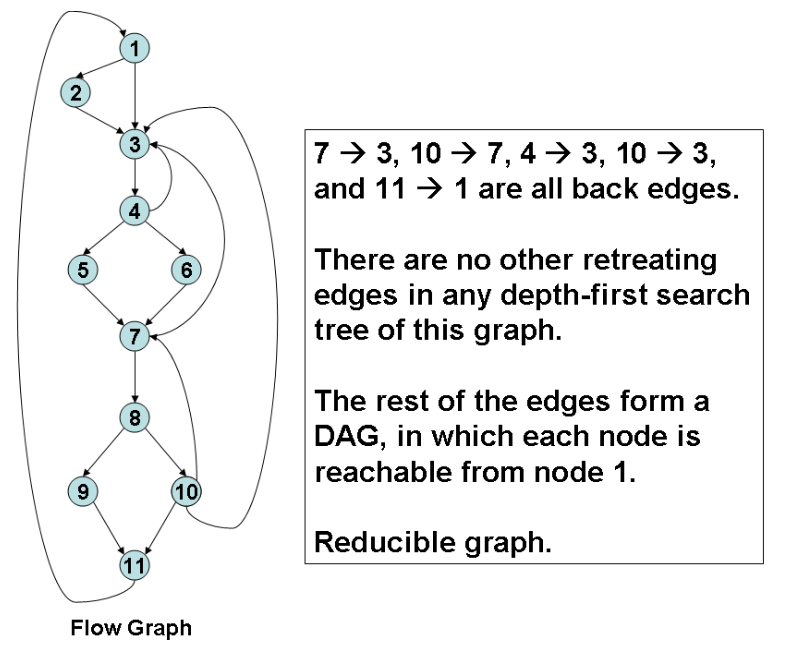
\includegraphics[width=0.4\textwidth]{Images/reducible.png}
    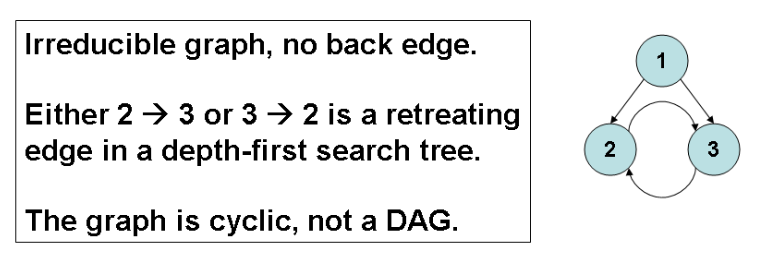
\includegraphics[width=0.4\textwidth]{Images/irreducible.png}
    \caption{Reducible and Irreducible CFG}
    \label{fig:cfg}
\end{figure}

\subsection*{Inner Loops}
Unless two loops have same header $n \longrightarrow d$ (here d is header), they are either disjoint or one is nested inside the other. If natural loop set of one header is subset of the other then there is nesting. Similarly two loops are disjoint if their natural loop sets are disjoint and two loops are identical if their natural loop sets are identical.

If two loops share a header, neither of these may hold and in such a case loops are combined and transformed.

\begin{figure}[h]
    \centering
    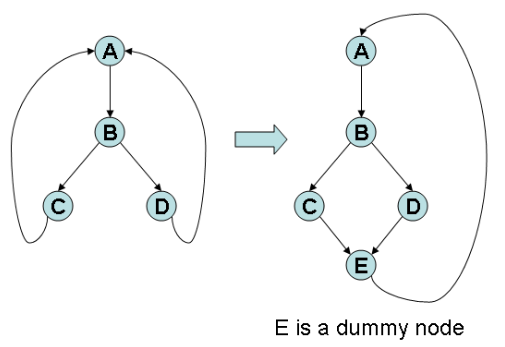
\includegraphics[width=0.4\textwidth]{Images/transform.png}
    \caption{Transformation in case of shared header}
    \label{fig:cfg}
\end{figure}]

\newpage

\subsection*{Pre Header}
\begin{figure}[h]
    \centering
    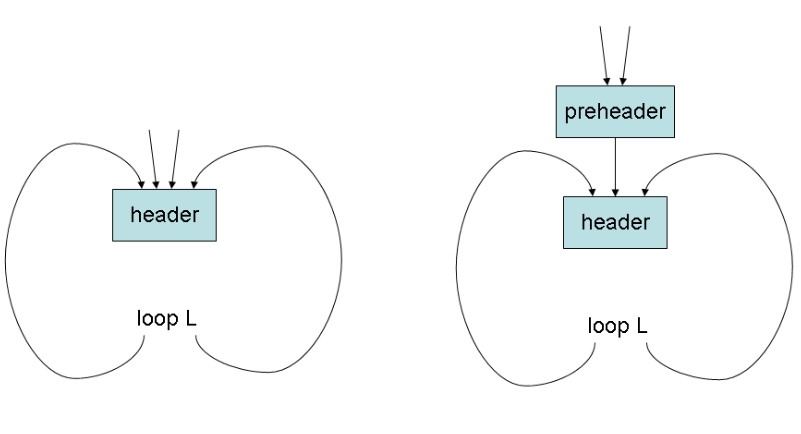
\includegraphics[width=0.4\textwidth]{Images/preheader.png}
    \caption{Pre Header}
    \label{fig:cfg}
\end{figure}

\subsection*{Depth of a CFG and Convergence of DFA Problem}
To be continued.

\end{document}
